\documentclass{article}
\usepackage{amsfonts}
\usepackage{graphicx}
\usepackage[margin=1in]{geometry}
\usepackage{bm}
\usepackage{amsmath}
\usepackage{authblk}
\usepackage{caption}
\usepackage{float}
\renewcommand{\familydefault}{\sfdefault}

\title{cILR: Taxonomic Enrichment Analysis with Isometric Log-Ratios}
\author[1,2]{Quang P. Nguyen}
\author[1,2]{Anne G. Hoen}
\author[1]{H. Robert Frost}
\affil[1]{Department of Biomedical Data Science, Geisel School of Medicine at Dartmouth College, Hanover, NH 03755, USA}
\affil[2]{Department of Epidemiology, Geisel School of Medicine at Dartmouth College, Hanover, NH 03755, USA}
\date{}                     %% if you don't need date to appear
\setcounter{Maxaffil}{0}
\renewcommand\Affilfont{\itshape\small}

\begin{document}
\maketitle
\captionsetup[figure]{labelfont={bf},name={Figure},labelsep=period, margin=2cm}

\begin{abstract}
    \noindent High-dimensionality and sparsity are challenging problems in statistical analysis of microbiome relative abundance data. One approach is to aggregate taxa to sets, most commonly to Linnean taxonomic categories identified through classification of representative sequences. However, most researchers perform aggregation through simple pairwise summation of counts. To address this issue, we developed a competitive set enrichment method based on the isometric log-ratio transformation (cILR) for microbiome relative abundance data. Our method generates sample-specific taxa set enrichment scores with a well-defined null hypothesis allowing for inference at both the sample and population levels. Here we demonstrated the performance of our method for multiple microbiome analysis tasks, including differential abundance testing and prediction. 
\end{abstract}

\section*{Background}
\section*{Methods}
\subsection*{Competitive Isometric Log-ratio (cILR)}
The cILR method generates sample-specific enrichment scores for microbial sets using the isometric log-ratio transformation \cite{egozcue2003}. The cILR method takes two inputs:  
\begin{itemize}
    \item $\mathbf{X}$: $n$ by $p$ matrix of positive counts for $p$ taxa and $n$ samples measured through either targeted sequencing (such as 16S rRNA) or whole genome shotgun sequening. Usually $\mathbf{X}$ is generated from standard sequence processing pipelines such as DADA2 \cite{callahan2016} and MetaPhlAn2 \cite{truong2015}. 
    \item $\mathbf{A}$: $p$ by $m$ indicator matrix annotating the membership of each taxa $p$ to $m$ sets of interest. These sets can be Linnean taxonomic classifications annotated using databases such as SILVA \cite{quast2013}, or those based on more functionally driven categories such as the tropism of each microbe ($a_{i,j} = 1$ indicates that microbe $i$ belongs to set $j$). 
\end{itemize}
The cILR method generates one output:  
\begin{itemize}
    \item $\mathbf{E}$: $n$ by $m$ matrix indicating the enrichment score of $m$ pre-defined sets identified in $\mathbf{A}$ across $n$ samples. 
\end{itemize}
The procedure is as follows:  
\begin{enumerate}
    \item \textbf{Compute the cILR statistic}: Let $\mathbf{M}$ be a $n$ by $m$ matrix of cILR scores. Let $\mathbf{M}_{i,k}$ be cILR scores for set $k$ of sample $i$:   
    $$\mathbf{M}_{i,k} = \sqrt{\frac{\sum_k A_{ik}(p - \sum_k A_{ik})}{p}} \ln \left( \frac{g(\mathbf{X}_{i,j}|\mathbf{A}_{j,k} = 1)}{g(\mathbf{X}_{i,j}|\mathbf{A}_{j,k} \neq 1))} \right)$$
    where $g()$ is the geometric mean. This represents the ratio of the geometric mean of the relative abundance of taxa assigned to set $k$ and remainder taxa.   
    \item \textbf{Compute the cILR statistic on permuted $\mathbf{X}$}: We seek to evaluate the empirical null distribution of the cILR statistic under $H_o$ that relative abundances in $\mathbf{X}$ of members of set $k$ are not enriched compared to those not in set $k$. Let $\mathbf{X}_p$ be the column permuted relative abundance matrix, and $\mathbf{M}_p$ be the corresponding cILR scores generated from $\mathbf{X}_p$. 
    \item \textbf{Fit Gaussian mixture distribution for each column of $\mathbf{M}_p$}
    \item \textbf{Calculate finalized cILR scores as CDF values of the fitted mixture distribution}
\end{enumerate}



\subsection*{Properties of cILR}
\subsubsection*{cILR and the Isometric Log Ratio Transformation}
Microbiome data is compositional \cite{gloor2017} and as such data transformation strategies from compositional data analysis (CoDA) \cite{aitchison} were often employed in analyses workflows. 
\subsubsection*{Null distribution of cILR}
\subsubsection*{Accounting for inter-taxa correlation}
Competitive enrichment tests, particularly those based on feature permutations, are sensitive to inter-feature correlations \cite{wu2012}. This is because the permutation procedure does not preserve the correlation structure, and any estimation based on the permuted null will underestimate the inflation in variance caused by

\subsection*{Simulation Design}

\section*{Results}
In this section we present the performance of our proposed method for three applicable microbiome analysis tasks: sample level enrichment, differential abundance, and prediction. We obtained these results from both parametric simulations and examples from real data.  
\subsection*{Enrichment testing at the sample level}
Our method provides a well-defined null hypothesis for significance testing at the sample level. Researchers who are interested in the enrichment of certain groups of microbes (for example, those of the \emph{Bifidobacterium} genus in infant gut microbiomes)  
\subsubsection*{Type I error control and power}
We benchmarked type I error on real stool microbiome data from HMP for both 16S and WGS type data. 16S data was taken from the package \emph{HMP16SData} snapshot 2020-10-02. 

\begin{figure}[H]
    \centering
    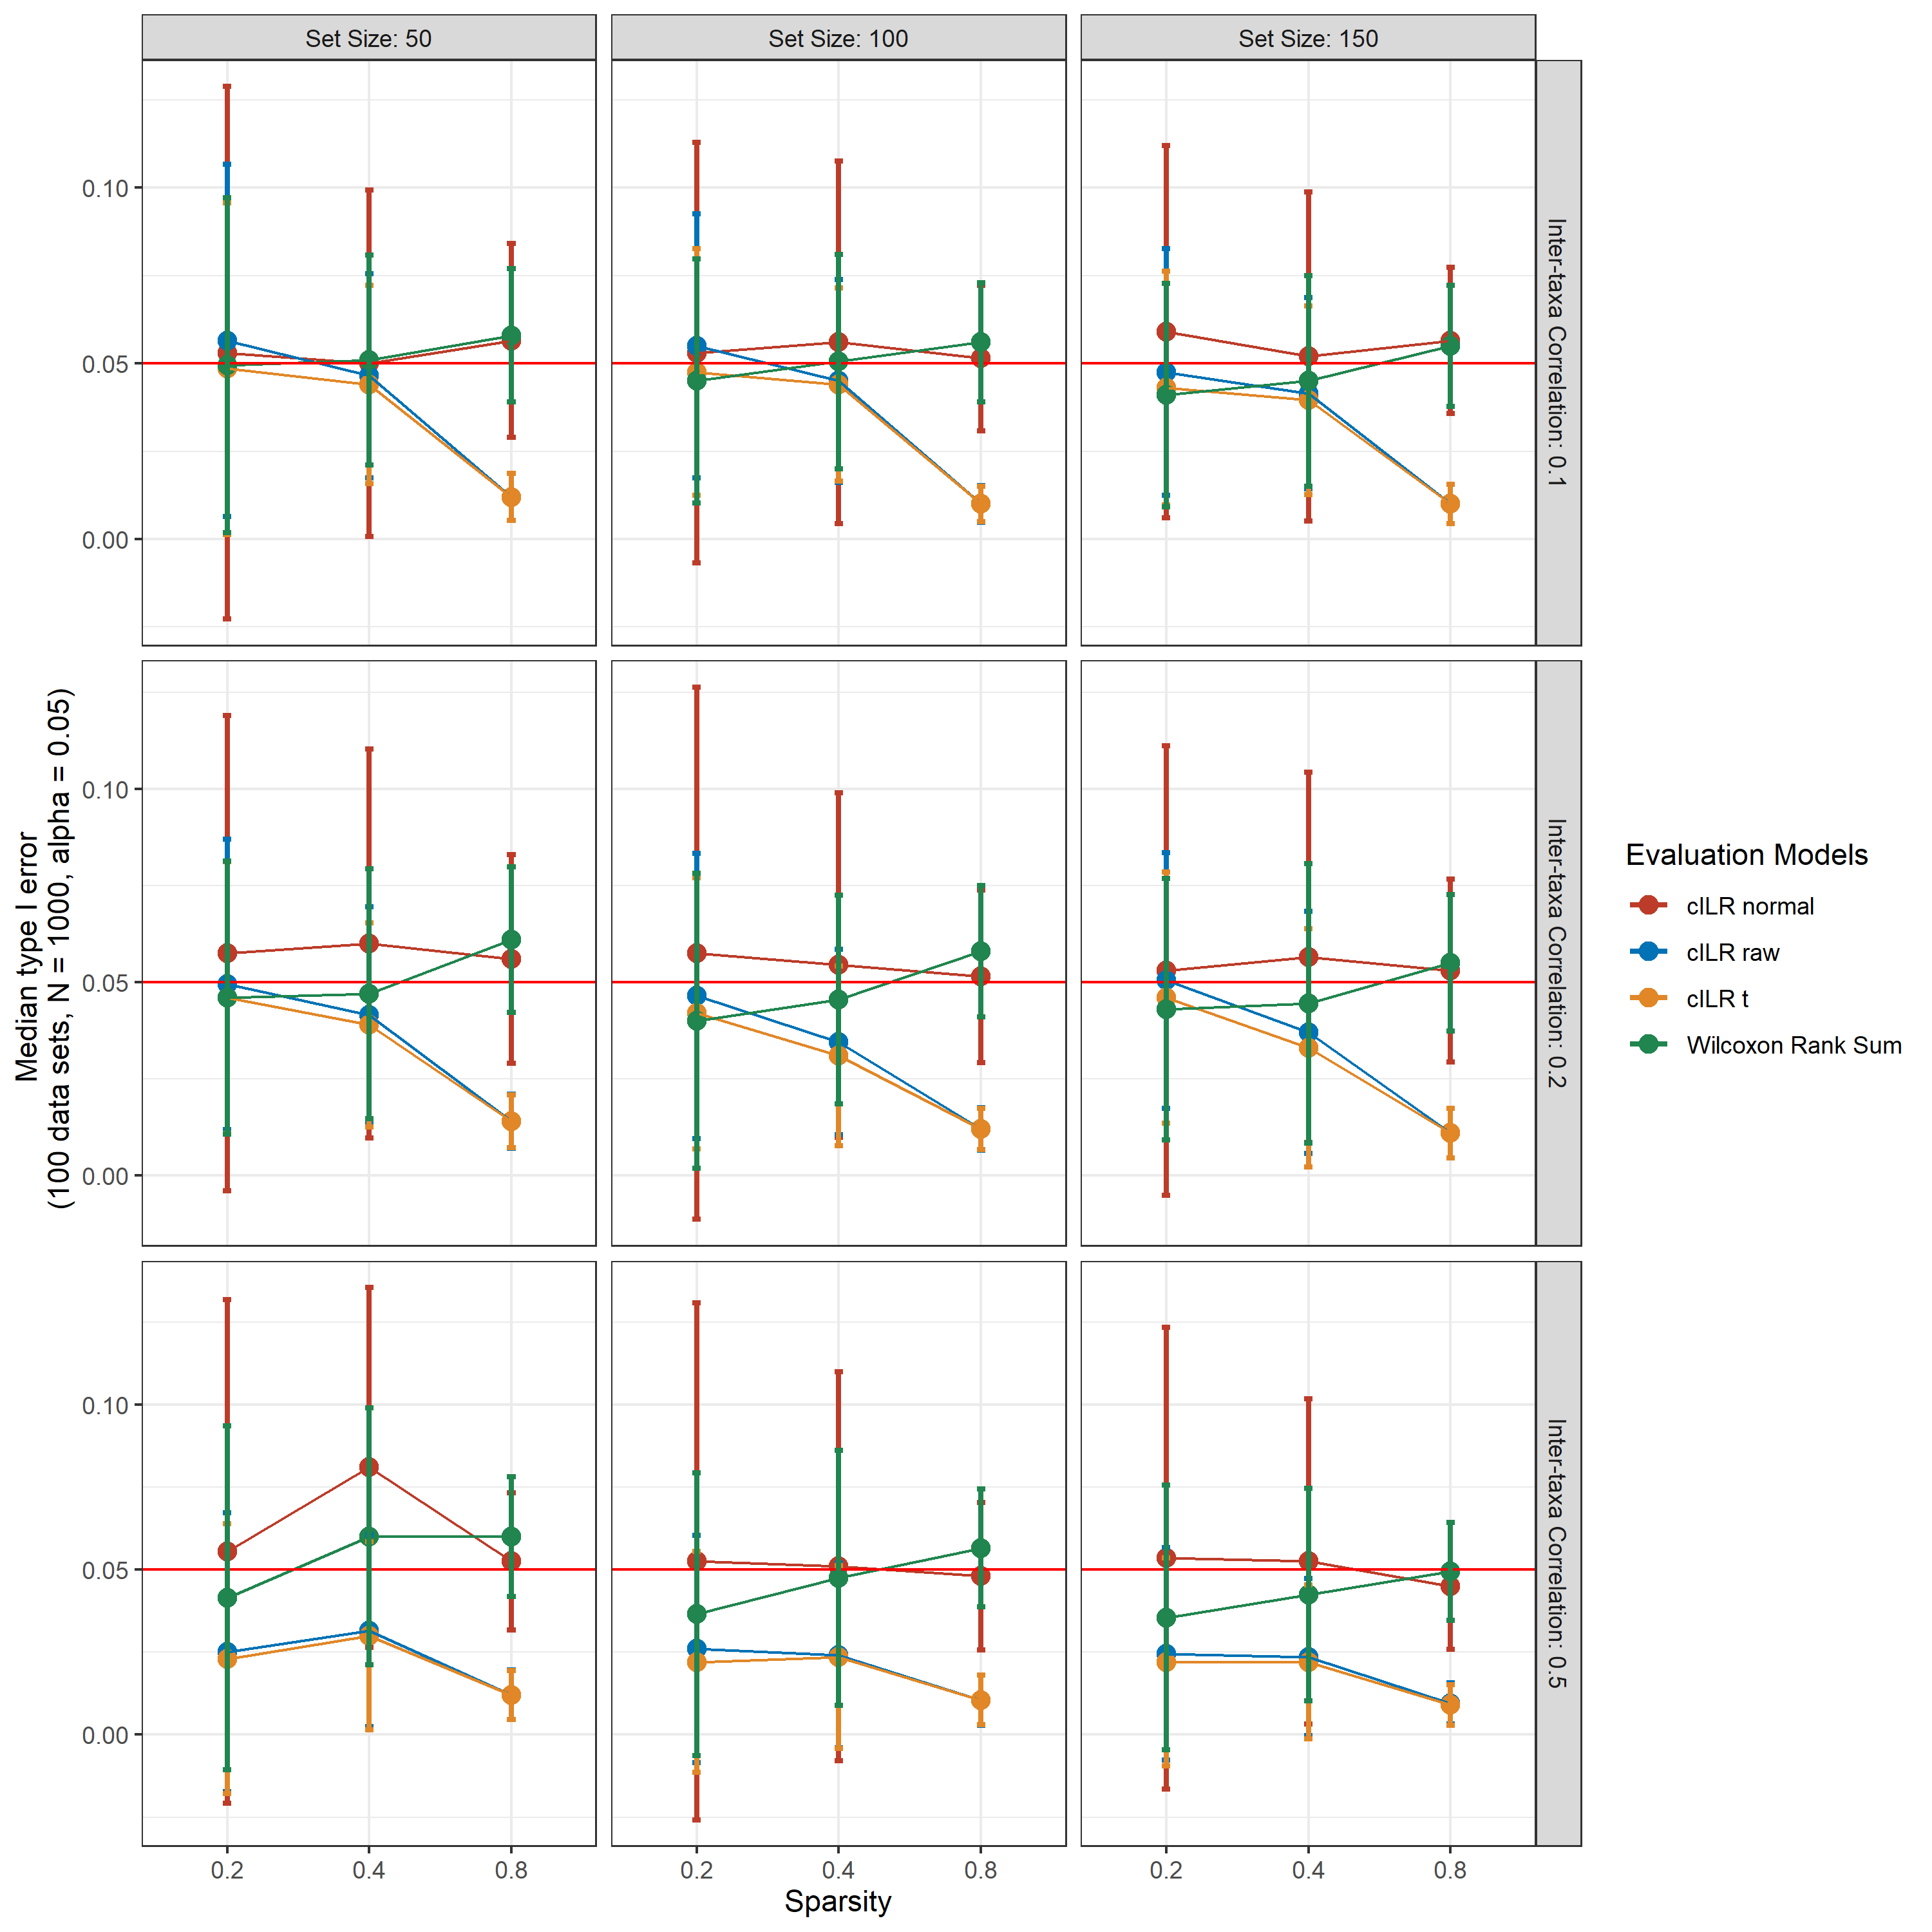
\includegraphics[scale = 0.4]{figures/fdr_single_sample.png}
    \caption{Median type I error rate as a function of data sparsity benchmarked on simulated null microbiome data as enumerated in SI methods. Enrichment of a specified set was tested at the sample level using cILR and the Wilcoxon rank sum test at $\alpha$ of 0.05. Each panel represents different in set size (horizontal) and inter-taxa correlation (vertical)}
\end{figure}

\begin{figure}[H]
    \centering
    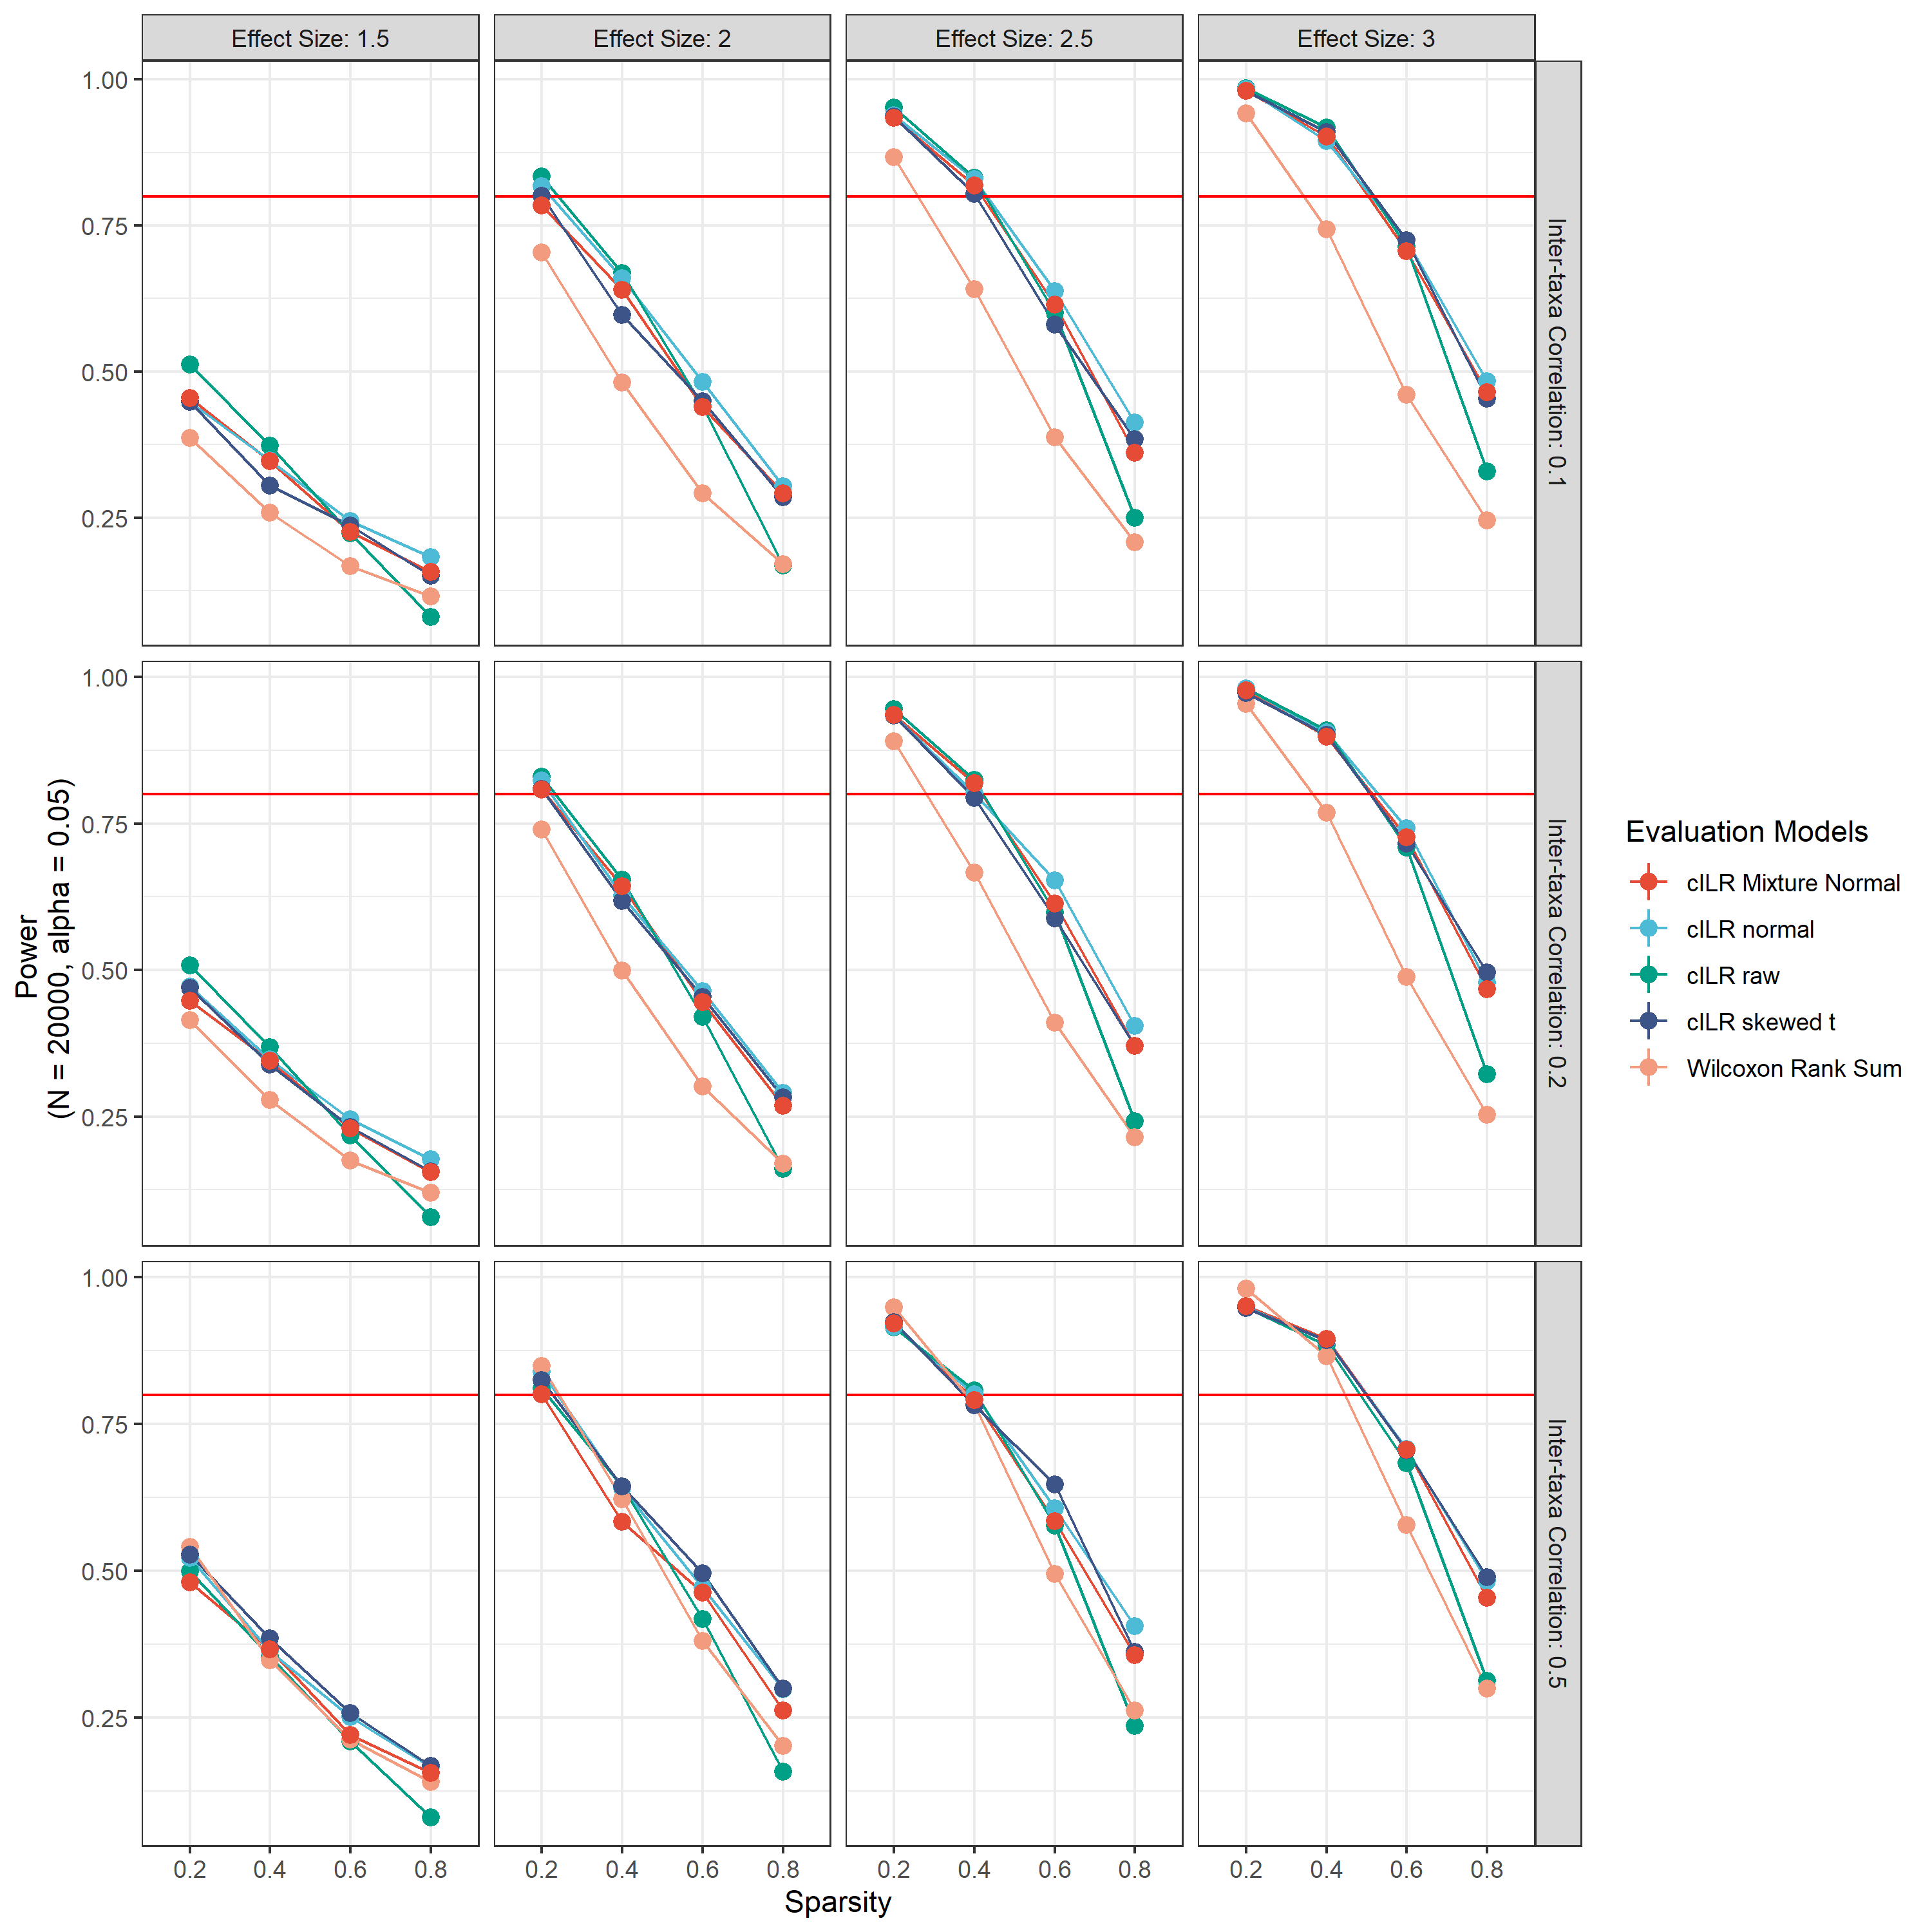
\includegraphics[scale=0.4]{figures/pwr_single_sample.png}
    \caption{Median power as a function of data sparsity benchmarked on simulated microbiome data as enumerated in SI Methods. Enrichment of a specified set was tested at the sample level using cILR and the Wilcoxon rank sum test at $\alpha$ of 0.05. Each panel represents different effect sizes (horizontal) and inter-taxa correlation (vertical).}
\end{figure}

\subsection*{Differential abundance analysis} 
\subsubsection*{Type I error control}
We benchmarked type I error rate of the cILR approach in differential abundance analysis tasks on both real data and numerical experiments. For real data, we utilized 16S rRNA and WGS stool sequencing data from the Human Microbiome project obtained from the packages \emph{HMP16SData} (ver. 1.9.3) and \emph{curatedMetagenomicData} in R. We randomly assigned samples from each data set into two arbitrary groups and evaluated the type I error rate. This procedure was repeated 1000 times. Figure 3 demonstrated these results.\\
We observed 
\begin{figure}[H]
    \centering
    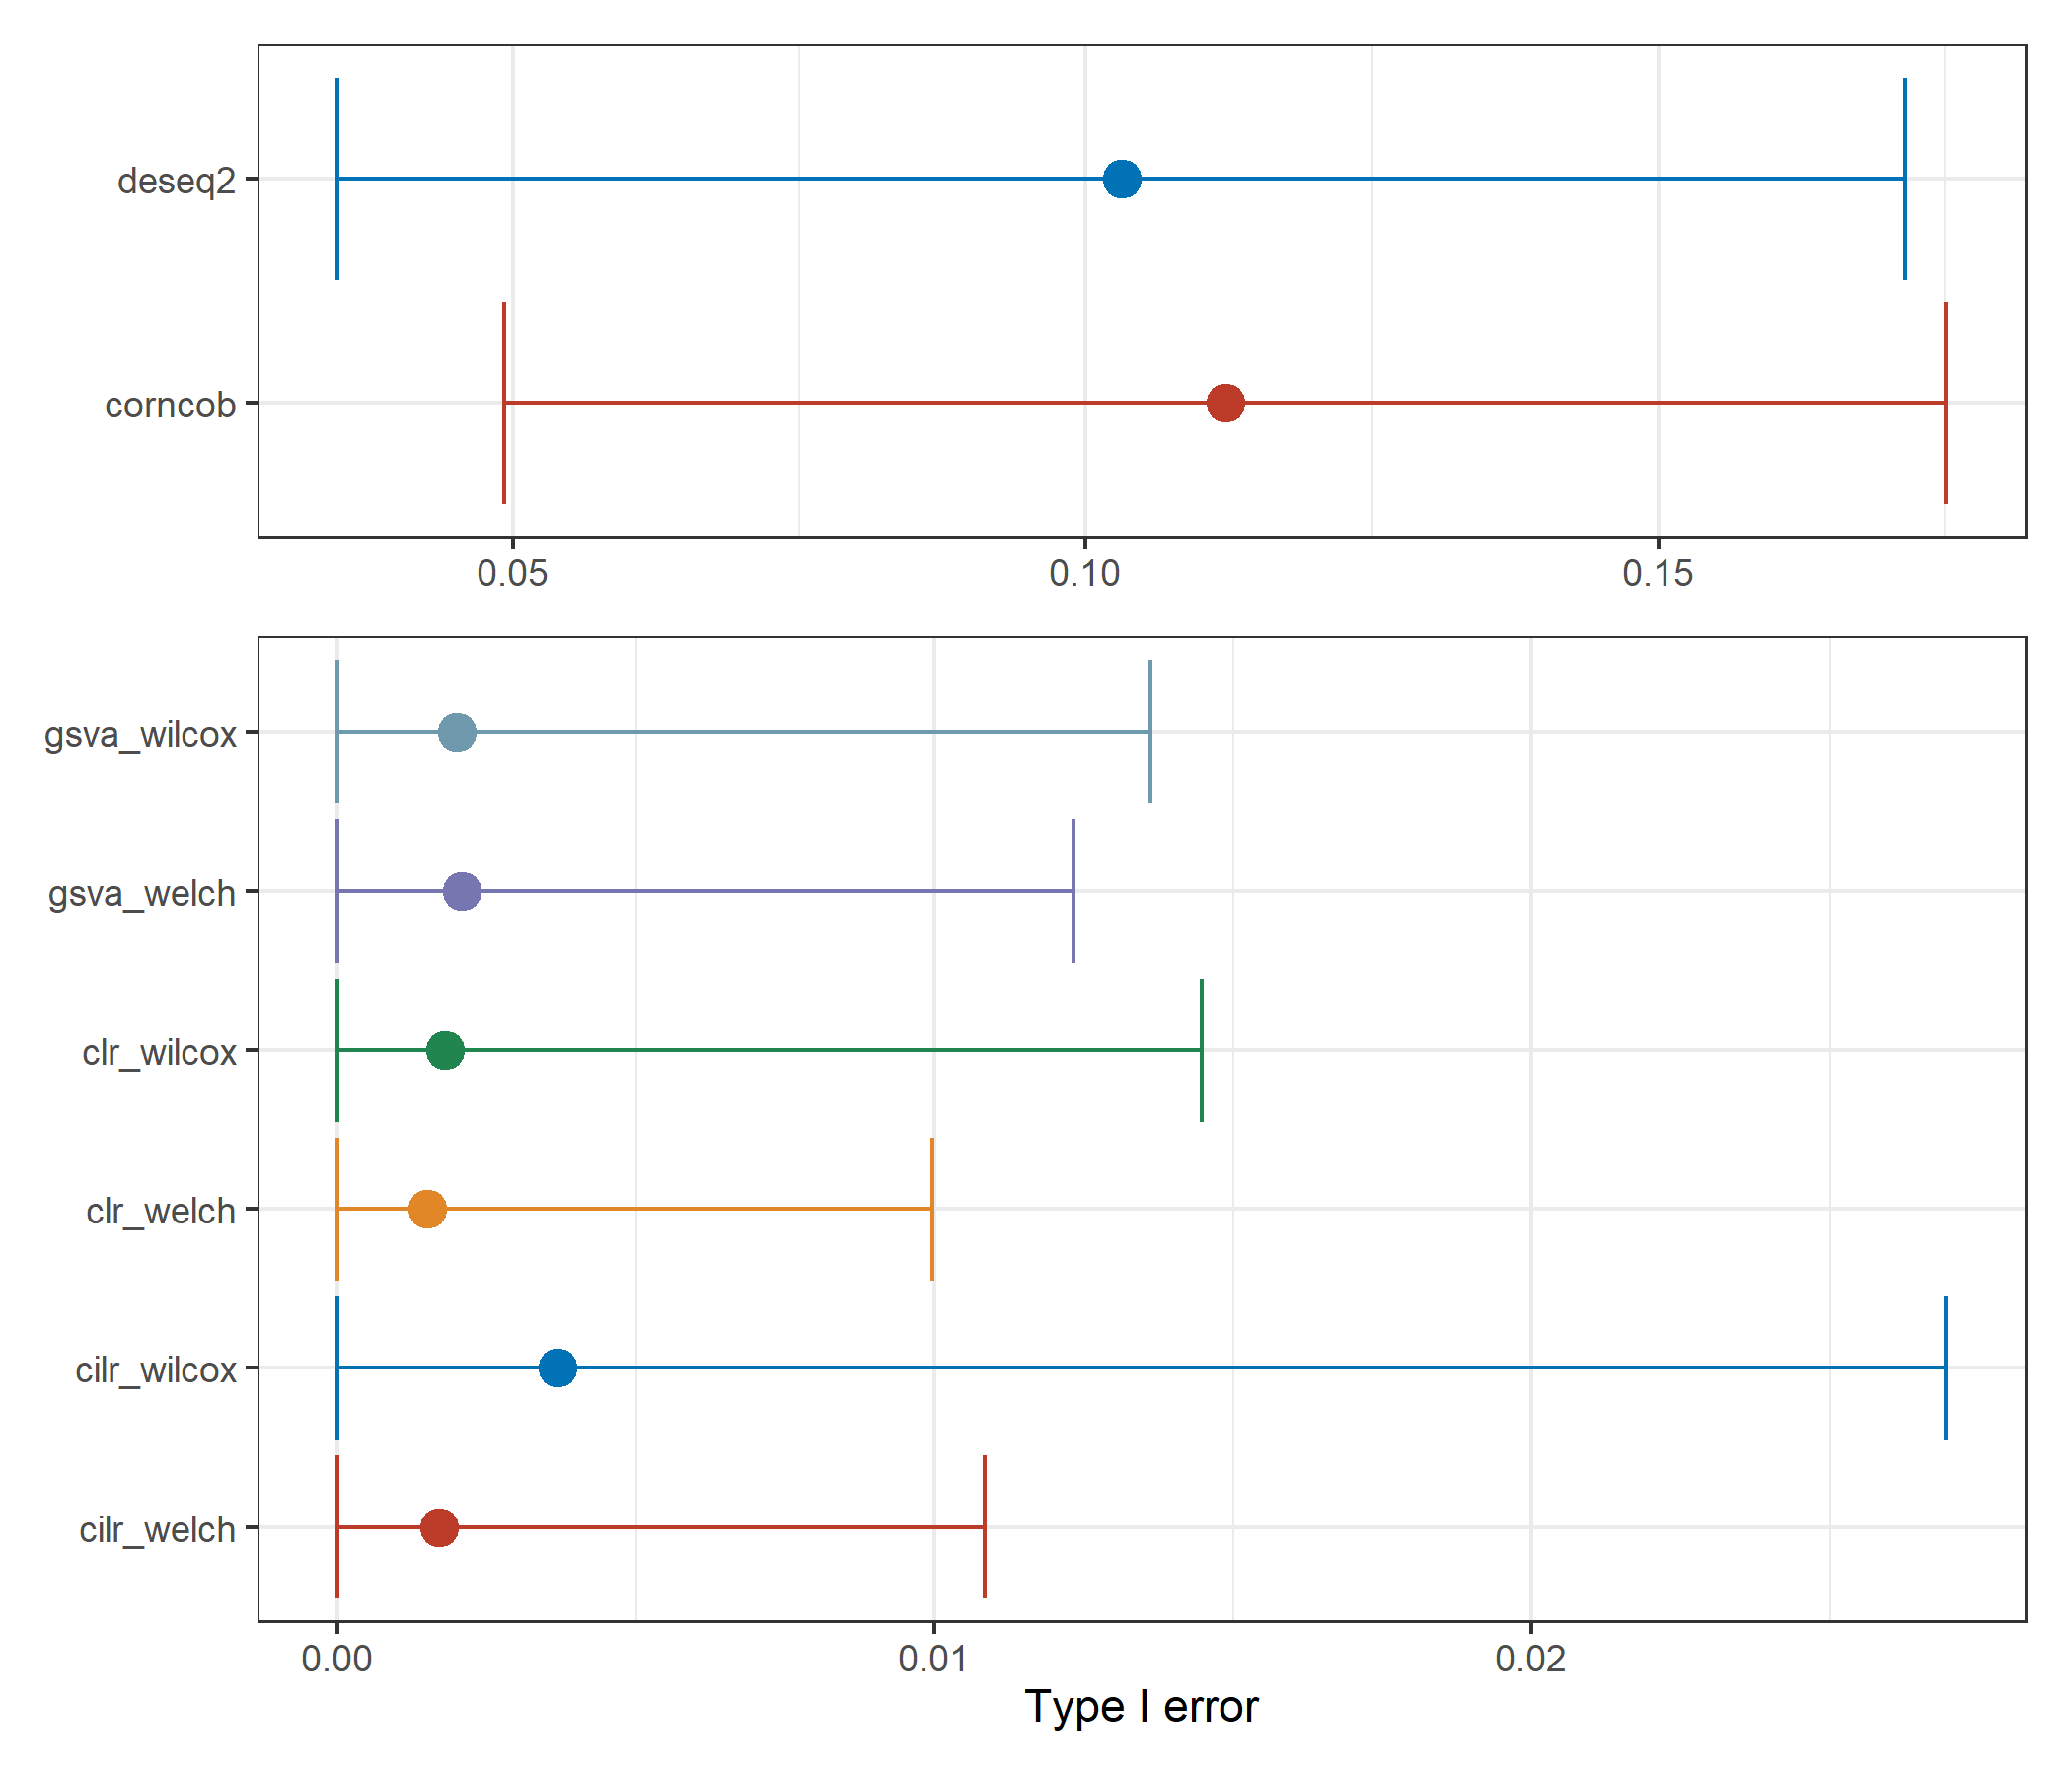
\includegraphics[scale=0.5]{figures/null_16s_da.png}
    \caption{Type I error evaluated on 16S rRNA and WGS stool samples obtained from HMP. Enrichment of genus level taxa sets was tested across different methods where significance was determined at FDR cutoff of 0.05.}
\end{figure}

\newpage
\bibliography{tax_agg}{}
\bibliographystyle{plain}
\end{document}
\end{document}